\documentclass[10pt, aspectratio=169]{beamer}
% \usepackage[T1]{fontenc} DO NOT ENABLE THIS!!!

\usetheme[progressbar=frametitle]{metropolis}
\usepackage{appendixnumberbeamer}
\setbeamertemplate{footline}{}
\setbeamertemplate{navigation symbols}[horizontal]

\setbeamertemplate{title page}{
    \begin{minipage}[c][\paperheight]{\textwidth}
        \ifx\inserttitlegraphic\@empty\else\usebeamertemplate*{title graphic}\fi
        \vfill%
        \ifx\inserttitle\@empty\else\usebeamertemplate*{title}\fi
        \ifx\insertsubtitle\@empty\else\usebeamertemplate*{subtitle}\fi
        \usebeamertemplate*{title separator}
        \begin{minipage}[t]{\textwidth}
            \ifx\beamer@shortauthor\@empty\else\usebeamertemplate*{author}\fi
            \ifx\insertdate\@empty\else\usebeamertemplate*{date}\fi
            \ifx\insertinstitute\@empty\else\usebeamertemplate*{institute}\fi
        \end{minipage}
        \vfill
        \vspace*{1mm}
    \end{minipage}
}

\metroset{sectionpage=none}
\setbeamertemplate{section in toc}[sections numbered]
\setbeamertemplate{subsection in toc}[subsections numbered]


\usepackage{booktabs}
\usepackage[scale=2]{ccicons}

\usepackage{amsmath}

\usepackage{float}

\usepackage{tabularx}
\usepackage{booktabs}

\usepackage{xcolor}
\definecolor{linkcolour}{rgb}{0,0.2,0.6}

\usepackage{hyperref}
\hypersetup{pdfauthor={Li, Binghuan}, 
            colorlinks,breaklinks,urlcolor=linkcolour, linkcolor=linkcolour}

\title{Approximation of the First Derivative}
\subtitle{Finite Difference Method\cite{Ferziger2002}}
\author{Binghuan W Li \ $\lvert$ \   \href{mailto:binghuan.li19@imperial.ac.uk}{binghuan.li19@imperial.ac.uk}}
\institute{Department of Bioengineering, Imperial College London}
\titlegraphic{\includegraphics[width=0.3\textwidth]{imgs/Imperial.eps}}



\begin{document}
\maketitle

\begin{frame}{Contents}
\tableofcontents
\end{frame}

\section{Definition of Derivatives}
\begin{frame}{Definition of Derivatives}
\[\bigg( \frac{\partial \phi}{\partial x}\bigg)_{x_{i}} = \lim_{\Delta x \to 0}\frac{\phi(x_{i}+\Delta x)-\phi(x_{i})}{\Delta x}\]
\begin{itemize}
    \item \textit{Forward}, \textit{backward} and \textit{central} difference:
\end{itemize}
    \begin{figure}[H]
        \centering
        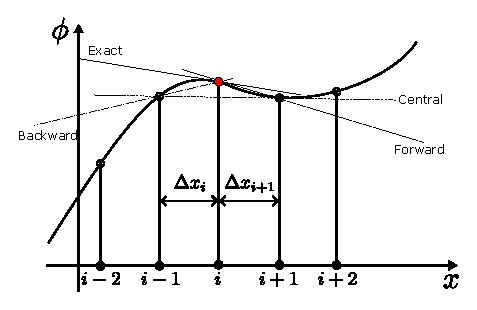
\includegraphics{imgs/def-of-derivative.eps}
        \caption{On the definition of derivatives and its approximations}
        \label{fig:my_label}
    \end{figure}
\end{frame}

\section{Taylor Series Expansion}
\begin{frame}{Taylor Series Expansion (1/)}
Taylor Series is defined as:
\begin{align*}
    \phi(x) &= 
    \phi(x_{i}) + (x-x_{i})\bigg(\frac{\partial \phi}{\partial x}\bigg)_{i}
    + \frac{(x-x_{i})^{2}}{2!}\bigg(\frac{\partial^{2} \phi}{\partial x^{2}}\bigg)_{i}  \\
    & +\frac{(x-x_{i})^{3}}{3!}\bigg(\frac{\partial^{3} \phi}{\partial x^{3}}\bigg)_{i} + ... 
    + \frac{(x-x_{i})^{n}}{n!}\bigg(\frac{\partial^{n} \phi}{\partial x^{n}}\bigg)_{i} + H
\end{align*}
where $H$ means \textit{higher order terms}.
\end{frame}

\begin{frame}{Taylor Series Expansion (2/)}
To find the first and higher derivatives of at point $x_{i}$ in terms of the function values at neighbouring points:
\begin{itemize}
    \item Forward:
    \[ \bigg(\frac{\partial \phi}{\partial x}\bigg)_{i} = 
    \frac{\phi_{i+1}-\phi_{i}}{x_{i+1}-x_{i}}
    - \frac{(x_{i+1}-x_{i})}{2}\bigg(\frac{\partial^{2} \phi}{\partial x^{2}}\bigg)_{i}
    -\frac{(x_{i+1}-x_{i})^{2}}{6}\bigg(\frac{\partial^{3} \phi}{\partial x^{3}}\bigg)_{i} + H\]   
    
    \item Backward:
    \[ \bigg(\frac{\partial \phi}{\partial x}\bigg)_{i} = 
    \frac{\phi_{i}-\phi_{i-1}}{x_{i}-x_{i-1}}
    + \frac{(x_{i}-x_{i-1})}{2}\bigg(\frac{\partial^{2} \phi}{\partial x^{2}}\bigg)_{i}
    -\frac{(x_{i}-x_{i-1})^{2}}{6}\bigg(\frac{\partial^{3} \phi}{\partial x^{3}}\bigg)_{i} + H\]  
    
    \item Central:
    \begin{align*}
    \bigg(\frac{\partial \phi}{\partial x}\bigg)_{i} &= 
    \frac{\phi_{i+1}-\phi_{i-1}}{x_{i+1}-x_{i-1}}
    - \frac{(x_{i+1}-x_{i})^{2} - (x_{i}-x_{i-1})^{2}}{2(x_{i+1}-x_{i-1})}\bigg(\frac{\partial^{2} \phi}{\partial x^{2}}\bigg)_{i}\\
    & -\frac{(x_{i+1}-x_{i})^{3} + (x_{i}-x_{i-1})^{3}}{6(x_{i+1}-x_{i-1})}\bigg(\frac{\partial^{3} \phi}{\partial x^{3}}\bigg)_{i} + H
    \end{align*}
\end{itemize}
\end{frame}

\begin{frame}{Taylor Series Expansion (3/)}
If the distance between the grids are infinitesimally small, \textit{i.e.} $x_{i}-x_{i-1}$ and $x_{i+1}-x_{i}$ are small enough: \textit{the first term dominates, neglect other terms}
\begin{itemize}
    \item Forward-difference scheme (FDS): \[ \bigg(\frac{\partial \phi}{\partial x}\bigg)_{i} = \frac{\phi_{i+1}-\phi_{i}}{x_{i+1}-x_{i}}\]
    \item Backward-difference scheme (BDS): \[ \bigg(\frac{\partial \phi}{\partial x}\bigg)_{i} = \frac{\phi_{i}-\phi_{i-1}}{x_{i}-x_{i-1}}\]
    \item Central-difference scheme (CDS): \[ \bigg(\frac{\partial \phi}{\partial x}\bigg)_{i} \approx \frac{\phi_{i+1}-\phi_{i-1}}{x_{i+1}-x_{i-1}}\]
\end{itemize}
\end{frame}

\begin{frame}{Taylor Series Expansion (4/)}
\textbf{Truncation errors} - the terms deleted from the right hand side.
\[\epsilon_{r} = (\Delta x)^{m}\alpha_{m+1} + (\Delta x)^{m+1}\alpha_{m+2} + ...+ (\Delta x)^{n}\alpha_{n+1}\]
where $\alpha$'s are higher-order derivatives multiplied by constant factors.
\end{frame}

\section{Polynomial Fitting}
% ======================================================

\begin{frame}{Polynomial Fitting (1/)}
\[\bigg( \frac{\partial \phi}{\partial x} \bigg)_{i} = \frac{\phi_{i+1}(\Delta x_{i})^{2} - \phi_{i-1}(\Delta x_{i+1})^{2} + \phi_{i}[(\Delta x_{i+1})^{2} - (\Delta x_{i})^{2}]}{\Delta x_{i+1}\Delta x_{i} (\Delta x_{i}+\Delta x_{i+1})} \]
where $\Delta x_{i} = x_{i} - x_{i-1}$.
\end{frame}

\section{Compact Schemes}

\begin{frame}{Compact Scheme - Pad\'e Approximation (1/)}
\begin{itemize}
    \item Assume: unform spaced grids
    \item Fourth-order Pad\`e scheme: use the variable values at $i$, $i+1$ and $i-1$:
    \[\phi = a_{0}+a_{1}(x-x_{i})+a_{2}(x-x_{i})^{2}+a_{3}(x-x_{i})^{3}+a_{4}(x-x_{i})^{4}\]
    \item We only need to compute $a_{1}$ - we are only interested in the first derivative.
    \[\frac{\partial \phi}{\partial x} = a_{1}+2a_{2}(x-x_{i})+ 3a_{3}(x-x_{i})^{2}+4a_{4}(x-x_{i})^{3} \approx a_{1}\]
    since we set $(x-x_{i})$ infinitesimally small.
\end{itemize}
\end{frame}

% ======================================================

\begin{frame}{Compact Scheme - Pad\'e Approximation (2/)}

\begin{itemize}
    \item Plug in $x=x_{i}$, $x=x_{i+1}$ and $x=x_{i-1}$ into:
    \begin{equation*}
        \boxed{\phi = a_{0}+a_{1}(x-x_{i})+a_{2}(x-x_{i})^{2}+a_{3}(x-x_{i})^{3}+a_{4}(x-x_{i})^{4}}
    \end{equation*}

    \item ... and plug in $x=x_{i+1}$ and $x=x_{i-1}$ into:
    \begin{equation*}
        \boxed{\frac{\partial \phi}{\partial x} = a_{1}+2a_{2}(x-x_{i})+ 3a_{3}(x-x_{i})^{2}+4a_{4}(x-x_{i})^{3} \approx a_{1}}
    \end{equation*}
    
    \item We got: 
    \[\bigg( \frac{\partial \phi}{\partial x}\bigg)_{i} = -\frac{1}{4}\bigg( \frac{\partial \phi}{\partial x}\bigg)_{i+1} - \frac{1}{4}\bigg( \frac{\partial \phi}{\partial x}\bigg)_{i-1} + \frac{3}{4}\frac{\phi_{i+1}-\phi_{i-1}}{\Delta x}\]
\end{itemize}
\end{frame}

% ======================================================

\begin{frame}{Compact Scheme - Pad\'e Approximation (3/)}

\begin{itemize}
    \item A family of compact centered approximations of up to sixth order can be written as:
    \[\alpha \bigg( \frac{\partial \phi}{\partial x}\bigg)_{i+1} + \bigg( \frac{\partial \phi}{\partial x}\bigg)_{i} + \alpha \bigg( \frac{\partial \phi}{\partial x}\bigg)_{i-1} = \beta \frac{\phi_{i+1}-\phi_{i-1}}{2\Delta x} + \gamma \frac{\phi_{i+2}-\phi_{i-2}}{4\Delta x}\]
    
    where $\alpha$, $\beta$ and $\gamma$ are three parameters which determine the second- and forth-order CDS and fourth- and sixth-order Pad\`e scheme.
\end{itemize}

\begin{table}[H]
    \centering
    \begin{tabular}{ccccc} \toprule
        Scheme      & Truncation error  & $\alpha$  & $\beta$   & $\gamma$ \\ \midrule
        CDS-2       & $\frac{(\Delta x)^{2}}{3!}\frac{\partial^{3}\phi}{\partial x^{3}}$    & 0 & 1 & 0 \\ [.5em]
        CDS-4       & $\frac{13(\Delta x)^{4}}{3 \cdot 3!}\frac{\partial^{5}\phi}{\partial x^{5}}$  & 0 & $\frac{4}{3}$ & $-\frac{1}{3}$ \\[.5em]
        Pad\`e-4    & $\frac{(\Delta x)^{4}}{5!}\frac{\partial^{5}\phi}{\partial x^{5}}$    & $\frac{1}{4}$ & $\frac{3}{2}$ & 0 \\[.5em]
        Pad\`e-6    & $\frac{4(\Delta x)^{6}}{7!}\frac{\partial^{7}\phi}{\partial x^{7}}$    & $\frac{1}{3}$ & $\frac{14}{9}$ & $\frac{1}{9}$ \\ \bottomrule
    \end{tabular}
    \caption{Compact Schemes: the parameters and truncation errors}
    \label{tab:my_label}
\end{table}
\end{frame}

\section{Non-Uniform Grids}
% ======================================================

\begin{frame}{Non-Uniform Grids (1/)}
\begin{itemize}
    \item \textbf{Problem} - cannot achieve a uniform distribution of discretization error on a uniform grid.
    \item \textbf{Solution} - use a smaller $\Delta x$ in regions where the derivatives of the function is large, and a larger $\Delta x$ when the function is smooth.
    \item \textbf{Aim} - spread the error nearly uniformly over the domain.
\end{itemize} 
\end{frame}

% ======================================================

\begin{frame}{Non-Uniform Grids (2/)}
\begin{itemize}
    \item Truncation error for the CDS is     
    \[
    \epsilon_{r} = 
    - \frac{(\Delta x_{i+1})^{2} - (\Delta x_{i})^{2}}{2(x_{i+1}-x_{i-1})}\bigg(\frac{\partial^{2} \phi}{\partial x^{2}}\bigg)_{i} + \frac{(\Delta x_{i+1})^{3} + (\Delta x_{i})^{3}}{6(x_{i+1}-x_{i-1})}\bigg(\frac{\partial^{3} \phi}{\partial x^{3}}\bigg)_{i} + H
    \]
    where $\Delta x_{i+1} = (x_{i+1}-x_{i})$ and $\Delta x_{i} = (x_{i}-x_{i-1})$. 
    
    \item \textbf{Assume} the grid expands or contracts with a constant factor $r_{e}$, known as a compound interest grid, we have: \[\Delta x_{i+1} = r_{e}\Delta x_{i}\]
    
    \item \textbf{Therefore}, the leading truncation error:
    \begin{itemize}
        \item For CDS: 
        \[
        \epsilon_{r} \approx
        \frac{(1-r_{e})\Delta x_{i}}{2}\bigg(\frac{\partial^{2}\phi}{\partial x^{2}}\bigg)_{i}
        \]
        \item For FDS and BDS (first-order):
        \[
        \epsilon_{r} \approx
        \frac{\Delta x_{i}}{2}\bigg(\frac{\partial^{2}\phi}{\partial x^{2}}\bigg)_{i}
        \]
    \end{itemize}
\end{itemize}
\end{frame}
%%=======================================================
\begin{frame}{Non-Uniform Grids (3/)}
 The leading truncation error:
    \begin{itemize}
        \item For CDS: 
        \[
        \epsilon_{r} \approx
        \frac{(1-r_{e})\Delta x_{i}}{2}\bigg(\frac{\partial^{2}\phi}{\partial x^{2}}\bigg)_{i}
        \]
        \item For FDS and BDS (first-order):
        \[
        \epsilon_{r} \approx
        \frac{\Delta x_{i}}{2}\bigg(\frac{\partial^{2}\phi}{\partial x^{2}}\bigg)_{i}
        \]
    \end{itemize}
From above, as $r_{e}$ is close to unity, the first-order truncation error of the CDS is substantially smaller than the FDS/BDS error.
\end{frame}
%%=======================================================
\begin{frame}{Non-Uniform Grids (4/)}
\begin{itemize}
    \item \textbf{Q:} what will happen when the grid is refined?
    \item Consider two scenarios: (1)\textbf{halving the spacing between two coarse grids} and (2)\textbf{inserting new points with a constant ratio of spacing}.
\end{itemize}
    
\metroset{block=fill}
\begin{block}{Scenario 1: halving the space}
    The spacing is uniform around new points with a constant $r_{e}$. If we repeat the refinement for several times, we can obtain a grid with uniform spacing \textit{almost} everywhere, except near the two coarsest points. Therefore, the CDS error vanishes.
\end{block}
\end{frame}
%%=======================================================
\begin{frame}[fragile]{Non-Uniform Grids (5/)}
\begin{figure}
    \centering
    \includegraphics[width=\textwidth]{imgs/non-uniform.eps}
    \caption{Refinement of a non-uniform grid}
    \label{fig:non-uniform}
\end{figure}

\metroset{block=fill}
\begin{block}{Scenario 2: inserting new points}\small
The expansion factor of the fine grid is smaller than on the coarse grid: $r_{e, h} = \sqrt{r_{e, 2h}}$, where $h$ represents the refined grid, and $2h$, the coarse grid. The ratio of the leading truncation error term at node $i$ on the two grids is:
    \[
    r_{\tau} = \frac{(1-r_{e})_{2h}(\Delta x_{i})_{2h}}{(1-r_{e})_{h}(\Delta x_{i})_{h}}
    \]
From \autoref{fig:non-uniform}:
    \[
    (\Delta x_{i})_{2h} = (\Delta x_{i})_{h} + (\Delta x_{i-1})_{h} = (r_{e}+1)_{h}(\Delta x_{i-1})_{h}
    \]
\end{block}
\end{frame}

%%=======================================================
\begin{frame}[fragile]{Non-Uniform Grids (6/)}
\metroset{block=fill}
\begin{block}{Scenario 2: inserting new points - CONT'D}\small
From \autoref{fig:non-uniform}:
    \[
    (\Delta x_{i})_{2h} = (\Delta x_{i})_{h} + (\Delta x_{i-1})_{h} = (r_{e}+1)_{h}(\Delta x_{i-1})_{h}
    \]
Therefore, the first-order truncation error of the CDS is reduced by a factor 
    \[
    r_{\tau} = \frac{(1+r_{e,h})^{2}}{r_{e,h}}
    \]
    When $r_{e} =1$, \textit{i.e.} when the grid is uniform, the factor $r_{\tau} = 4$; When $r_{e} < 1$ or $r_{e} > 1$, \textit{i.e.} the grid is contacting or expanding, the factor $r_{\tau}>4$. This means that the error due to the first-order term decreases faster than the second-order error term.
\end{block}
\textbf{Conclusion:} systematic refinement of non-uniform grids gives a rate of reduction of truncation error that has the same order as for a uniform gird.
\end{frame}

%%=======================================================
\begin{frame}[fragile]{Non-Uniform Grids (7/)}
\metroset{block=fill}
Higher order approximation of the first derivative can be obtained by using more points to eliminate more of the truncation error terms. For example, using $\phi_{i-1}$ to obtain an expression for the second derivative at $x_{i}$:
    \begin{align*}
    \bigg( \frac{\partial \phi}{\partial x} \bigg)_{i} 
    & = \frac{\phi_{i+1}(\Delta x_{i})^{2}-\phi_{i-1}(\Delta x_{i+1})^{2} + \phi_{i}[(\Delta x_{i+1})^{2}-(\Delta x_{i})^{2}]}{\Delta x_{i+1}\Delta x_{i}(\Delta x_{i}+\Delta x_{i+1})} \\
    & - \frac{\Delta x_{i+1}\Delta x_{i}}{6}\bigg( \frac{\partial^{3} \phi}{\partial x^{3}} \bigg)_{i} + H
    \end{align*}
\end{frame}


% COMMENT OUT BUT LEAVE HERE AS ILLUSTRATION ON PURPOSE!!
% \begin{frame}{Page111} 

% \begin{alertblock}{123123123}
%  test test test
%  As this titleformat also uses smallcaps you face the same problemsas with thesmallcapstitleformat. Additionally this format cancause some other problems. Please refer to the documentation ifyou consider using it.As a rule of thumb: Just use it for plaintext-only titles.
%  \end{alertblock}
% \end{frame}

% \begin{frame}{Page222}
% \metroset{block=fill}
%  \begin{exampleblock}{Example here}
%  As this titleformat also uses smallcaps you face the same problemsas with thesmallcapstitleformat. Additionally this format cancause some other problems. Please refer to the documentation ifyou consider using it.As a rule of thumb: Just use it for plaintext-only titles.
%  \end{exampleblock}
% \end{frame}

\appendix

\begin{frame}{Reference}
 \bibliography{bibTeX/ferziger.bib}
 \bibliographystyle{abbrv}
\end{frame}

\end{document}
